%-----------------------------------------------------------------------------%
\chapter{\babTiga}
%-----------------------------------------------------------------------------%
Pada bagian ini akan dijelaskan metodologi yang digunakan dalam penelitian. Metodologi ini mencakup metode implementasi OpenCL untuk masing-masing operasi serta metode eksperimen.

\section{Metode Implementasi }
%-----------------------------------------------------------------------------%
Pada penelitian ini penulis memanfaatkan Tensorflow Lite untuk menjalankan \textit{Deep Learning inference} pada perangkat \textit{mobile}. Tensorflow Lite memiliki \textit{kernel} tersendiri yang terpisah dari \textit{core} Tensorflow.  Penulis memodifikasi Tensorflow Lite \textit{kernel} dengan menambahkan implementasi OpenCL untuk operasi perkalian matriks-matriks, perkalian matriks-vektor, dan konvolusi matriks sehingga operasi-operasi tersebut dapat dijalankan pada GPU ketika \textit{inference} berlangsung. Implementasi OpenCL pada tiga operasi tersebut hanya dapat digunakan oleh \textit{fully-connected} layer dan \textit{convolution layer}.

Tensorflow Lite telah memiliki dua jenis Tensorflow Lite \textit{kernel} untuk operasi matriks pada \textit{convolution layer} dan \textit{fully-connected layer}, yaitu \textit{naive kernel} dan \textit{optimized kernel}, dimana keduanya dijalankan pada CPU. Dengan menambahkan Tensorflow Lite \textit{kernel} yang diimplementasikan melalui OpenCL, ada tiga jenis Tensorflow Lite \textit{kernel} yang dapat digunakan. Saat kompilasi, pengguna dapat memilih untuk menggunakan \textit{naive kernel} (CPU), \textit{optimized kernel} (CPU), atau OpenCL \textit{kernel} (GPU). \pic~\ref{fig:modifieddiagram} menunjukkan bagaimana penulis memodifikasi Tensorflow Lite \textit{kernel}.

\begin{figure}
	\centering
	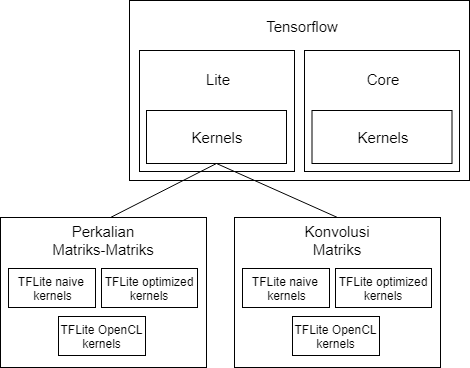
\includegraphics[width=0.50\textwidth]
	{pics/modifieddiagram.png}
	\caption{Modifikasi Tensorflow Lite \textit{kernel} dengan menambahkan satu jenis \textit{kernel} baru untuk operasi perkalian matriks-matriks dan konvolusi matriks yang diimplementasikan melalui OpenCL dan berjalan di GPU.}
	\label{fig:modifieddiagram}
\end{figure}

Persiapan-persiapan OpenCL seperti yang disebutkan pada BAB II memerlukan cukup banyak waktu. Untuk mengurangi biaya persiapan yang mahal, beberapa persiapan tidak dilakukan pada setiap \textit{inference}, namun hanya dilakukan satu kali pada awal berjalannya aplikasi \textit{Deep Learning}. Hal ini dilakukan dengan cara meletakkan persiapan-persiapan tersebut pada \textit{interpreter} sehingga persiapan tersebut hanya dilakukan ketika Tensorflow Lite melakukan interpretasi model. Objek-objek hasil dari persiapan OpenCL seperti \textit{context} dan \textit{buffer} tersebut kemudian dapat diberikan sebagai argumen ketika melakukan interpretasi \textit{fully-connected layer} dan \textit{convolution layer}. Ketika \textit{inference}, objek \textit{fully-connected layer} dan \textit{convolution layer} pada Tensorflow Lite dapat menggunakan objek-objek OpenCL yang telah dipersiapkan di awal. Persiapan untuk OpenCL yang dilakukan pada awal berjalannya aplikasi dapat dilihat pada \tab~\ref{tab:SetupCL}.

\begin{table}
	\centering
	\caption{Persiapan OpenCL yang dilakukan satu kali pada awal berjalannya aplikasi.}
	\label{tab:SetupCL}
	\begin{tabular}{| l | l |}
		\hline
		\textbf{No.} & \textbf{Persiapan OpenCL} \\ 
		\hline
		1 & Membuat \textit{context} \\ 
		\hline 
		2 & Membuat \textit{command queue} \\ 
		\hline 
		3 & Membuat \textit{kernel} \\ 
		\hline
		4 & Membuat \textit{buffer} \\ 
		\hline
	\end{tabular}
\end{table}

Persiapan yang tidak dapat dilakukan hanya satu kali adalah menyalin data masukan operasi \textit{inference} dari memori CPU ke memori GPU. Proses menyalin data ini harus dikerjakan pada setiap \textit{inference} karena data masukan bersifat dinamis. Perhatikan \pic~\ref{fig:initcl} dan \pic~\ref{fig:copydata} untuk mengetahui lebih jelas bagaimana persiapan untuk OpenCL dilakukan pada penelitian ini.

\begin{figure}
	\centering
	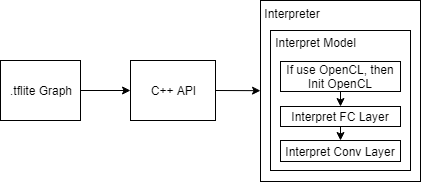
\includegraphics[width=0.50\textwidth]
	{pics/initcl.png}
	\caption{Metode persiapan untuk OpenCL yang dilakukan hanya satu kali di awal berjalannya suatu aplikasi \textit{Deep Learning}. Persiapan dilakukan ketika \textit{interpreter} melakukan inisiasi model.}
	\label{fig:initcl}
\end{figure}

\begin{figure}
	\centering
	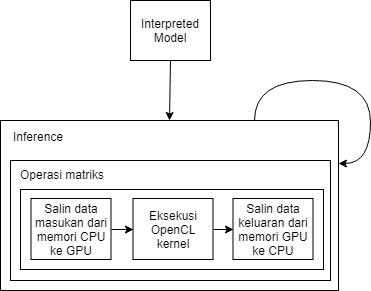
\includegraphics[width=0.50\textwidth]
	{pics/copydata.png}
	\caption{Proses menyalin data masukan dan keluaran antara memori CPU dan GPU dilakukan pada setiap \textit{inference}. Proses menyalin data tidak dapat dilakukan satu kali saja karena data bersifat dinamis.}
	\label{fig:copydata}
\end{figure}

\subsection{Metode Implementasi Konvolusi Matriks }
Operasi konvolusi matriks memiliki dua matriks masukan, yaitu \textit{image} dan \textit{filter}, dan satu matriks keluaran yaitu matriks \textit{output}. Matriks-matriks tersebut merupakan matriks empat dimensi yaitu kanal, baris, kolom, dan \textit{batch}. Seluruh matriks masukan dan keluaran disimpan di memori GPU secara linear dengan struktur seperti pada \pic~\ref{fig:linearconv}. Semua matriks menggunakan tipe data vektor $float4$. Apabila banyaknya kanal dari matriks bukan kelipatan empat, maka diberikan \textit{padding} pada struktur linear di memori GPU tersebut sedemikian sehingga setiap vektor $float4$ mengandung elemen-elemen yang merupakan elemen-elemen matriks pada kolom, baris, dan \textit{batch} yang sama. 

\begin{figure}
	\centering
	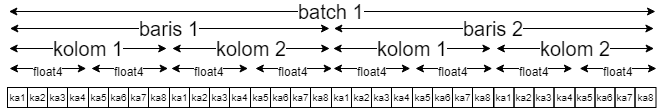
\includegraphics[width=0.50\textwidth]
	{pics/linearconv.png}
	\caption{Struktur linear matriks masukan dan keluaran yang disimpan di memori GPU untuk operasi konvolusi. Elemen ke-15 dari data linear tersebut adalah elemen pada kanal ke-7, kolom ke-2, baris ke-1 dan \textit{batch} ke-1 dari matriks.}
	\label{fig:linearconv}
\end{figure}

Misalkan banyaknya kanal, tinggi, lebar, dan banyaknya \textit{batch} dari \textit{image}, \textit{filter}, dan \textit{output} berturut-turut adalah $C_i \times H_i \times W_i \times B_i$, $C_f \times H_f \times W_f \times B_f$, dan $C_o \times H_o \times W_o \times B_o$. Pada implementasi ini digunakan \textit{work-space} dua dimensi berukuran $H_{ws} \times W_{ws}$ dan \textit{work-group} dua dimensi berukuran $H_{wg} \times W_{wg}$ dengan $H_{ws} = H_o' \times B_o$ dan $W_{ws} = W_o' \times ceil(C_o/4)$, dimana $Wo'$ adalah bilangan kelipatan $W_{wg}$ terkecil yang lebih besar atau sama dengan $W_o$ dan $H_o'$ adalah bilangan kelipatan $H_{wg}$ terkecil yang lebih besar atau sama dengan $H_o$. \pic~\ref{fig:wiconv} merupakan contoh struktur \textit{work-space} dengan $H_{wg} = 8$ dan $W_{wg} = 32$.

\begin{figure}
	\centering
	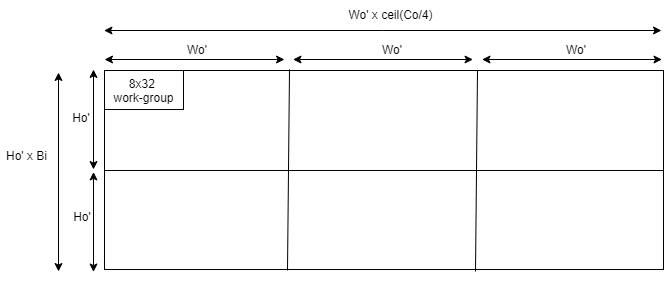
\includegraphics[width=0.50\textwidth]
	{pics/wiconv.png}
	\caption{Struktur \textit{work-space} untuk konvolusi matriks. Dalam kasus ini $W_o$ adalah kelipatan 32 dan $H_o$ adalah kelipatan 8.}
	\label{fig:wiconv}
\end{figure}

Dengan struktur tersebut, setiap vektor $float4$ pada matriks \textit{output} dikomputasi oleh suatu \textit{work-item} yang unik. Selain itu, suatu \textit{work-group} melakukan komputasi untuk memperoleh satu blok matriks \textit{output} dengan tinggi, lebar, dan banyaknya kanal $H_{wg} \times W_{wg} \times 4$. Blok tersebut merupakan hasil konvolusi dari suatu blok lain pada matriks \textit{image} dengan tinggi, lebar, dan banyaknya kanal $(H_{wg}+H_f-1) \times (W_{wg}+W_f-1) \times C_i$ dengan empat \textit{filter} yang berbeda. Ini dapat dilihat pada \pic~\ref{fig:convblock}.   

\begin{figure}
	\centering
	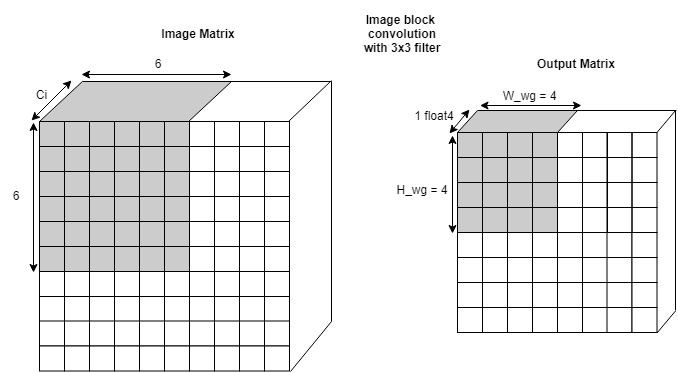
\includegraphics[width=0.50\textwidth]
	{pics/convblock.png}
	\caption{Blok pada matriks \textit{output} yang dikomputasi oleh suatu \textit{work-group}. Blok tersebut terdiri dari empat kanal. Blok berwarna abu-abu pada matriks \textit{output} merupakan hasil konvolusi dari blok abu-abu dari matriks \textit{image}.}
	\label{fig:convblock}
\end{figure}

Perhatikan bahwa untuk memperoleh satu blok matriks \textit{output}, hampir semua elemen pada blok matriks \textit{image} akan diakses lebih dari satu kali oleh \textit{work-group}. Mengetahui fakta ini, penulis menggunakan \textit{local memory caching} untuk mengurangi redundansi akses ke \textit{global memory}. Konvolusi untuk suatu blok matriks \textit{output} dilakukan dalam $ceil(C_i/4)$ iterasi, dimana setiap iterasi hanya melibatkan blok matriks \textit{image} yang berukuran $(H_{wg}+H_f-1) \times (W_{wg}+W_f-1) \times 4$ seperti yang dapat dilihat pada \pic~\ref{fig:conviter}. Hasil konvolusi dari semua iterasi kemudian diakumulasikan. Dengan menggunakan \textit{local memory caching}, pada setiap iterasi blok matriks \textit{image} ini disalin terlebih dahulu dari \textit{global memory} ke \textit{local memory} sebelum digunakan untuk komputasi. Setiap \textit{work-item} pada \textit{work-group} bertugas menyalin maksimal empat vektor $float4$ dari blok matriks \textit{image} ke \textit{local memory} seperti yang terlihat pada \pic~\ref{fig:convlocal}.  

\begin{figure}
	\centering
	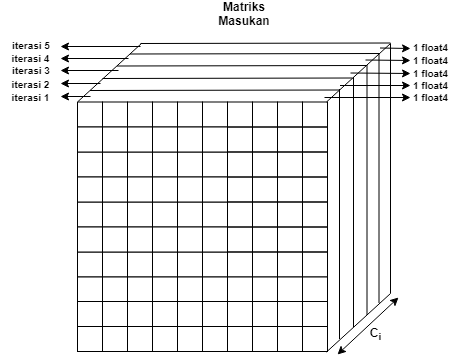
\includegraphics[width=0.50\textwidth]
	{pics/conviter.png}
	\caption{Operasi konvolusi dilakukan dalam $ceil(C_i/4)$ iterasi dimana $C_i$ adalah kedalaman \textit{image}. Setiap iterasi melibatkan blok matriks \textit{image} dengan kedalaman 4, sesuai dengan panjang vektor $float4$.}
	\label{fig:conviter}
\end{figure}

\begin{figure}
	\centering
	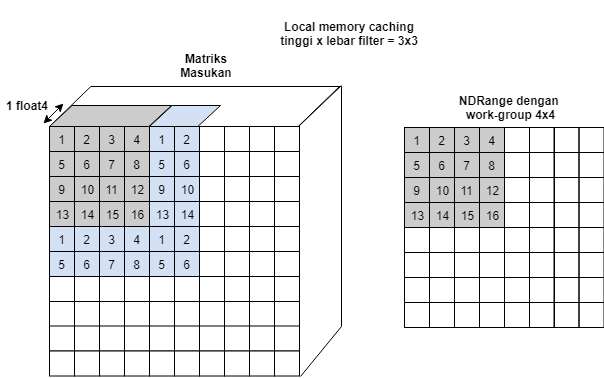
\includegraphics[width=0.50\textwidth]
	{pics/convlocal.png}
	\caption{\textit{Local memory cahing} terhadap matriks \textit{image} pada suatu iterasi dalam kasus \textit{filter} berukuran panjang dan lebar $3 \times 3$. \textit{Work-item} dengan nomor $i$ bertugas menyalin vektor-vektor $float4$ dari \textit{image} dengan nomor $i$ ke local memory.}
	\label{fig:convlocal}
\end{figure}

\subsection{Metode Implementasi Perkalian Matriks-Matriks }
Dalam pembahasan ini dimisalkan matriks masukan adalah matriks A dan matriks B, sedangkan matriks keluaran adalah matriks C. Sama seperti konvolusi, seluruh matriks disimpan secara linear di memori GPU. Matrix A dan matriks C disimpan secara \textit{row-major}, sedangkan matrix B disimpan secara \textit{column-major} seperti pada \pic~\ref{fig:linearmatmat}.  Semua matriks menggunakan tipe data vektor $float4$. Jika lebar dari matriks A atau C bukan kelipatan 4, maka diberikan \textit{padding} pada struktur linear di memori GPU sedemikian sehingga setiap vektor $float4$ mengandung elemen-elemen yang merupakan elemen-elemen matriks pada baris yang sama. Untuk matriks B, \textit{padding} diberikan jika tingginya bukan kelipatan 4.

\begin{figure}
	\centering
	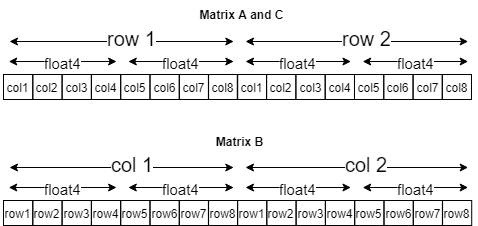
\includegraphics[width=0.50\textwidth]
	{pics/linearmatmat.png}
	\caption{Struktur linear matriks A, B, dan C pada operasi perkalian matriks-matriks. A dan C disimpan secara \textit{row-major}, sedangkan B secara \textit{column-major}.}
	\label{fig:linearmatmat}
\end{figure}

Misalkan matriks A berukuran $M \times K$ dan matriks B berukuran $K \times N$, maka matriks C berukuran $M \times N$. Untuk menjalankan operasi perkalian matriks-matriks di GPU, digunakan \textit{work-space} dua dimensi dengan ukuran $H_{ws} \times W_{ws}$ dan \textit{work-group} dua dimensi berukuran $H_{wg} \times W_{wg}$ dimana $H_{ws}$ adalah bilangan kelipatan $H_{wg}$ terkecil yang lebih besar atau sama dengan $M$ dan $W_{ws}$ adalah bilangan kelipatan $W_{wg}$ terkecil yang lebih besar atau sama dengan $ceil(N/4)$. Untuk ukuran \textit{work-group}, berlaku aturan $H_{wg} = 4 \times W_{wg}$. 

\begin{figure}
	\centering
	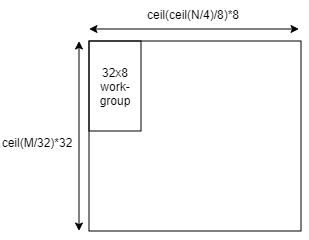
\includegraphics[width=0.50\textwidth]
	{pics/wimatmat.png}
	\caption{Struktur \textit{work-space} untuk perkalian matriks-matriks. Dalam kasus ini tinggi \textit{work-space} adalah kelipatan 32 dan lebarnya adalah kelipatan 8.}
	\label{fig:wimatmat}
\end{figure}

Dengan struktur di atas, setiap vektor $float4$ pada matriks C dikomputasi oleh satu \textit{work-item} yang unik. Lalu, masing-masing \textit{work-group} melakukan komputasi untuk memperoleh satu blok pada matriks C yang berukuran $H_{wg} \times H_{wg}$ seperti pada \pic~\ref{fig:wimatmat}. Perhatikan bahwa setiap blok matriks C tersebut diperoleh dari perkalian matriks antara dua blok lain, yaitu satu blok dari matriks A berukuran $H_{wg} \times K$ dan satu blok dari matriks B berukuran $K \times H_{wg}$. \pic~\ref{fig:blackmatmat} adalah contoh perkalian antara dua blok matriks untuk menghasilkan blok berukuran $32 \times 32$ pada matriks C ketika ukuran \textit{work-group} adalah $32 \times 8$.

\begin{figure}
	\centering
	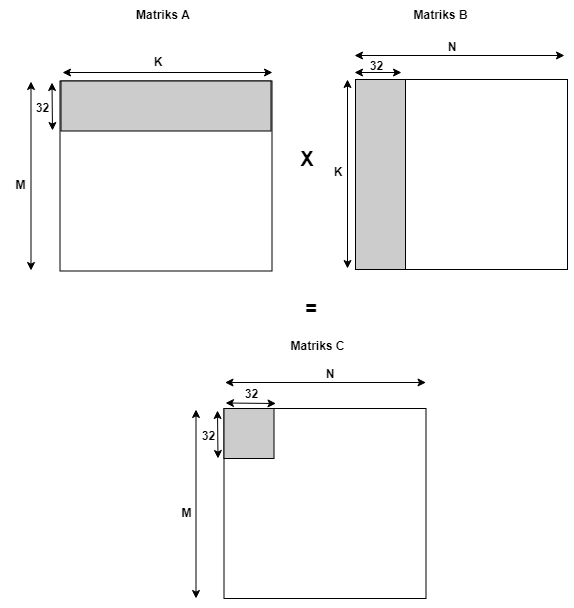
\includegraphics[width=0.50\textwidth]
	{pics/blockmatmat.png}
	\caption{Perkalian antara dua blok $32 \times K$ dan $K \times 32$ pada matriks A dan B sehingga menghasilkan satu blok $32 \times 32$ pada matriks C. Ukuran work-group dalam kasus ini adalah $32 \times 8$.}
	\label{fig:blockmatmat}
\end{figure}

Seperti pada konvolusi, perkalian dua blok matriks tersebut juga mengandung redundansi akses \textit{global memory} karena elemen-elemen yang sama pada blok diakses lebih dari satu kali. Penulis juga menggunakan \textit{local memory caching} dalam implementasi ini. Perkalian antar dua blok matriks A dan B dilakukan dalam $ceil(K/H_{wg})$ iterasi. Pada setiap iterasi, dilakukan perkalian dua blok yang berukuran lebih kecil yaitu antara blok $H_{wg} \times H_{wg}$ dari matriks A dengan blok $H_{wg} \times H_{wg}$ dari matriks B seperti pada \pic~\ref{fig:matmatiter}. Hasil perkalian dari semua iterasi kemudian diakumulasikan. Pada setiap iterasi, masing-masing \textit{work-item} pada \textit{work-group} berutgas menyalin dua vektor $float4$, satu dari blok matriks A dan satu dari blok matriks B, ke \textit{local memory} seperti yang terlihat pada \pic~\ref{fig:localmatmat} sebelum komputasi dilakukan.

\begin{figure}
	\centering
	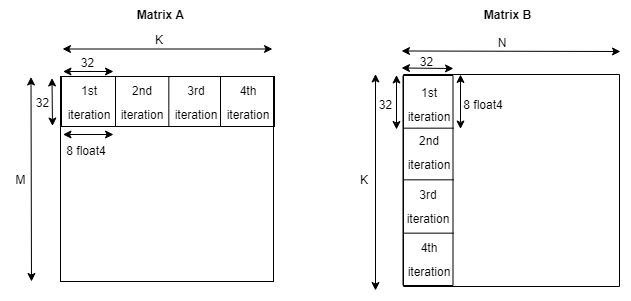
\includegraphics[width=0.50\textwidth]
	{pics/matmatiter.png}
	\caption{Operasi perklaian matriks-matriks yang dilakukan dalam $ceil(K/32)$ iterasi pada kasus ukuran work-group $32 \times 8$. Setiap iterasi melibatkan blok matriks A dengan lebar 32 dan blok matriks B dengan tinggi 32.}
	\label{fig:matmatiter}
\end{figure}

\begin{figure}
	\centering
	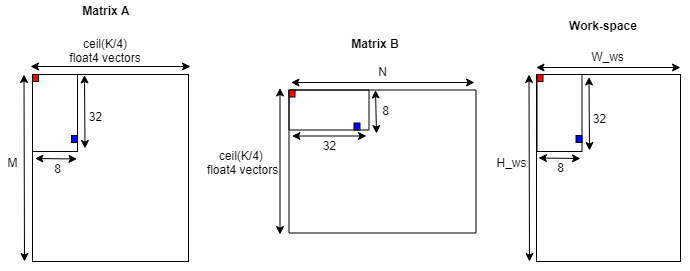
\includegraphics[width=0.50\textwidth]
	{pics/localmatmat.png}
	\caption{Pembagian kerja untuk menyalin blok matriks A dan B dari \textit{global memory} ke \textit{local memory} pada \textit{work-group} dengan ukuran $32 \times 8$. Masing-masing \textit{work-item} menyalin dua vektor $float4$. \textit{Work-item} merah memuat vektor berwarna merah dan \textit{work-item} biru memuat vektor berwarna biru.}
	\label{fig:localmatmat}
\end{figure}

\section{Metode Eksperimen }
%-----------------------------------------------------------------------------%
Eksperimen dilakukan terhadap masing-masing jenis Tensorflow Lite \textit{kernel} untuk operasi perkalian matriks-matriks dan konvolusi matriks, yaitu Tensorflow Lite \textit{naive kernel} yang berjalan di CPU, Tensorflow Lite \textit{optimized kernel} yang berjalan di CPU, dan Tensorflow Lite OpenCL \textit{kernel} yang berjalan di GPU. Dalam eksperimen ini penulis mengukur kecepatan eksekusi tiga \textit{kernel} tersebut pada berbagai kasus dan ukuran matriks atau vektor masukan. Hasil pengukuran kecepatan dari masing-masing \textit{kernel} kemudian dibandingkan. Untuk Tensorflow Lite OpenCL \textit{kernel}, penulis melakukan dua jenis pengukuran kecepatan. Pertama, pengukuran dilakukan terhadap eksekusi OpenCL \textit{kernel} saja (komputasi saja). Kedua, pengukuran dilakukan terhadap komputasi OpenCL beserta persiapan OpenCL yang diperlukan pada setiap \textit{inference}, yaitu proses menyalin data antar memori CPU dan GPU. Dengan demikian, penulis dapat mengetahui pada apakah \textit{bottleneck} dari OpenCL terletak pada transfer data antar memori atau terletak pada komputasi. Untuk menghitung kecepatan dari suatu Tensorflow Lite \textit{kernel} penulis menggunakan \textit{wall-clock time} dengan cara menghitung selisih dari \textit{wall-clock time} sebelum dan sesudah Tensorflow Lite \textit{kernel} berjalan.